\documentclass[aspectratio=169]{beamer}

\mode<presentation>
{
  \usetheme{default}
  \usecolortheme{default}
  \usefonttheme{default}
  \setbeamertemplate{navigation symbols}{}
  \setbeamertemplate{caption}[numbered]
  \setbeamertemplate{footline}[frame number]  % or "page number"
  \setbeamercolor{frametitle}{fg=white}
  \setbeamercolor{footline}{fg=black}
} 

\usepackage[english]{babel}
\usepackage[utf8x]{inputenc}
\usepackage{tikz}
\usepackage{courier}
\usepackage{array}
\usepackage{bold-extra}
\usepackage{minted}
\usepackage[thicklines]{cancel}

\xdefinecolor{dianablue}{rgb}{0.18,0.24,0.31}
\xdefinecolor{darkblue}{rgb}{0.1,0.1,0.7}
\xdefinecolor{darkgreen}{rgb}{0,0.5,0}
\xdefinecolor{darkgrey}{rgb}{0.35,0.35,0.35}
\xdefinecolor{darkorange}{rgb}{0.8,0.5,0}
\xdefinecolor{darkred}{rgb}{0.7,0,0}
\definecolor{darkgreen}{rgb}{0,0.6,0}
\definecolor{mauve}{rgb}{0.58,0,0.82}

\title[2018-07-10-chep-columnar]{Columnar data processing for HEP analysis}
\author{Jim Pivarski}
\institute{Princeton University -- DIANA-HEP}
\date{July 10, 2018}

\begin{document}

\logo{\pgfputat{\pgfxy(0.11, 7.4)}{\pgfbox[right,base]{\tikz{\filldraw[fill=dianablue, draw=none] (0 cm, 0 cm) rectangle (50 cm, 1 cm);}\mbox{\hspace{-8 cm}\includegraphics[height=1 cm]{princeton-logo-long.png}\includegraphics[height=1 cm]{diana-hep-logo-long.png}}}}}

\begin{frame}
  \titlepage
\end{frame}

\logo{\pgfputat{\pgfxy(0.11, 7.4)}{\pgfbox[right,base]{\tikz{\filldraw[fill=dianablue, draw=none] (0 cm, 0 cm) rectangle (50 cm, 1 cm);}\mbox{\hspace{-8 cm}\includegraphics[height=1 cm]{princeton-logo.png}\includegraphics[height=1 cm]{diana-hep-logo.png}}}}}

% Uncomment these lines for an automatically generated outline.
%\begin{frame}{Outline}
%  \tableofcontents
%\end{frame}

% START START START START START START START START START START START START START

\begin{frame}{First slide}
\vspace{0.5 cm}
HERE
\end{frame}

\begin{frame}{Landscape of vertical performance}
\vspace{0.3 cm}
\begin{columns}
\column{1.15\linewidth}
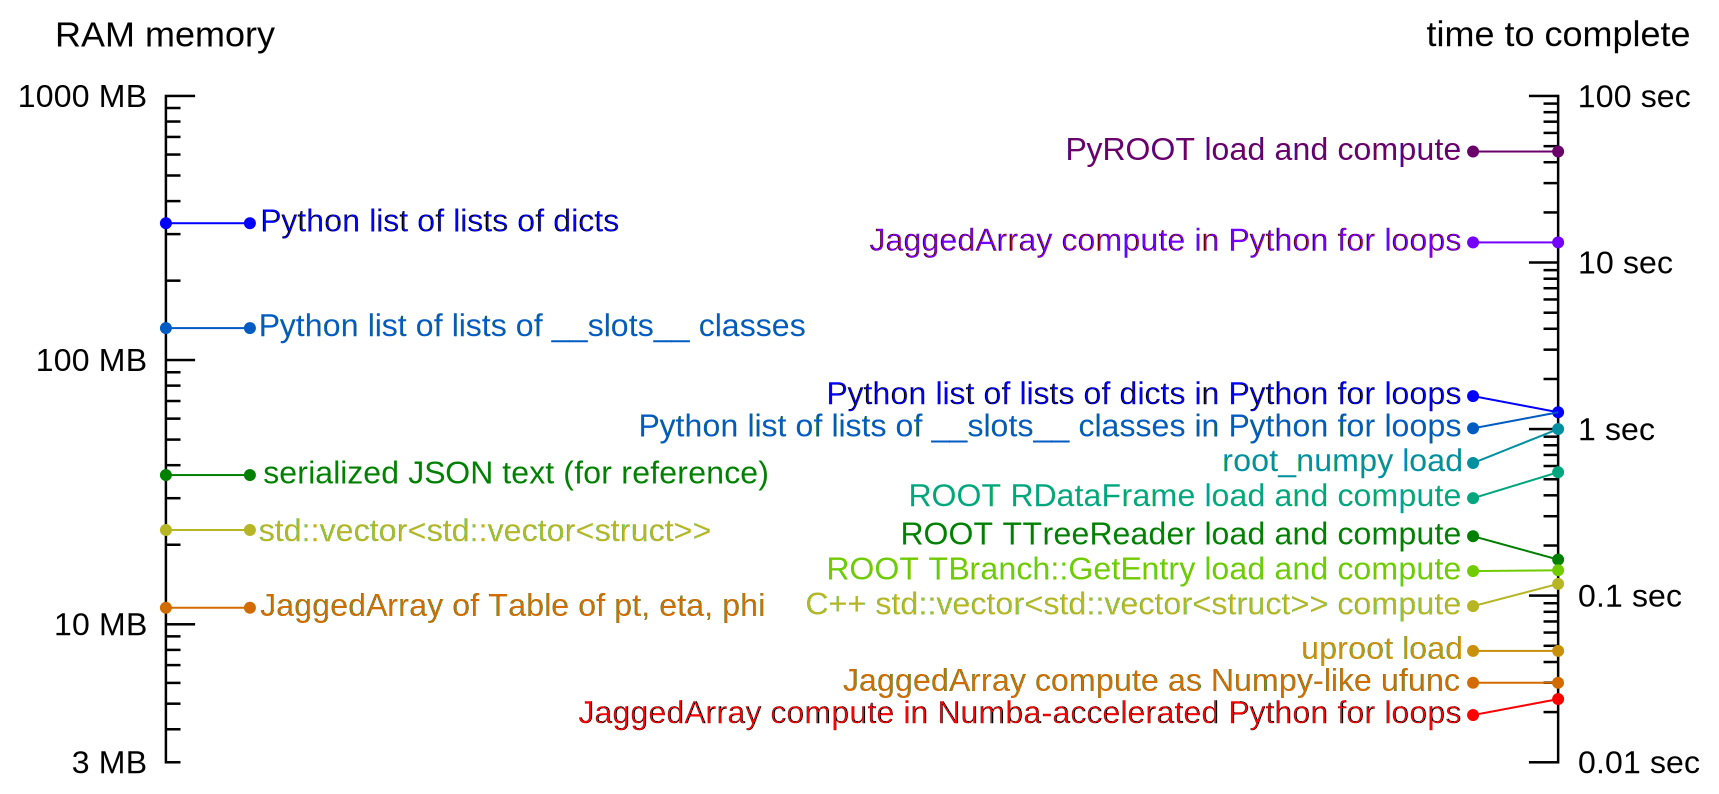
\includegraphics[width=\linewidth]{logscales.pdf}
\end{columns}
\end{frame}

\begin{frame}{Landscape of vertical performance}
\vspace{0.3 cm}
\scriptsize

\begin{columns}
\column{1.1\linewidth}
\begin{columns}
\column{0.38\linewidth}
\begin{tabular}{r p{0.9\linewidth}}
& \textcolor{darkblue}{\underline{RAM memory occupied by data (MB)}} \\
& \\
311.95 & Python list of lists of dicts \\
139.79 & Python list of lists of {\tt\scriptsize \_\_slots\_\_} classes \\
& \\
 37.19 & serialized JSON text (for reference) \\
& \\
 22.38 & {\tt\scriptsize std::vector<std::vector<struct>>} \\
 11.67 & JaggedArray of Table of pt, eta, phi \\
\end{tabular}

\column{0.6\linewidth}
\begin{tabular}{r p{0.9\linewidth}}
& \textcolor{darkblue}{\underline{time to complete load, compute, or both (sec)}} \\
& \\
45.9\textcolor{white}{00} & PyROOT load and compute \\
& \\
 1.79\textcolor{white}{0} & JaggedArray compute in Python for loops \\
 1.24\textcolor{white}{0} & Python list of lists of dicts in Python for loops \\
 1.23\textcolor{white}{0} & Python list of lists of {\tt\scriptsize \_\_slots\_\_} classes in Python for loops \\
& \\
 0.770 & root\_numpy load \\
& \\
 0.538 & ROOT RDataFrame load and compute \\
 0.164 & ROOT TTreeReader load and compute \\
 0.142 & ROOT TBranch::GetEntry load and compute \\
 0.113 & C++ {\tt\scriptsize std::vector<std::vector<struct>>} compute \\
& \\
 0.047 & uproot load \\
 0.030 & JaggedArray compute as Numpy-like ufunc \\
 0.023 & JaggedArray compute in Numba-accelerated Python for loops \\
\end{tabular}
\end{columns}
\end{columns}
\end{frame}


\end{document}
